\subsection{Estado del Arte}

\subsubsection{Migración de plataformas Firebase hacia arquitecturas en AWS}

Como lo indica J. Michel \cite{Michael2021}, Firebase ofrece una arquitectura de dos capas, donde las aplicaciones cliente (web o móviles) interactúan directamente con servicios \textit{backend} como Firestore, Authentication y Cloud Functions. Esta simplicidad facilita el desarrollo rápido de MVPs, pero puede presentar desafíos en escalabilidad, control y flexibilidad a medida que la aplicación crece. Obsérvese la \autoref{fig:firebase_architecture}.

\begin{figure}[H]
  \centering
  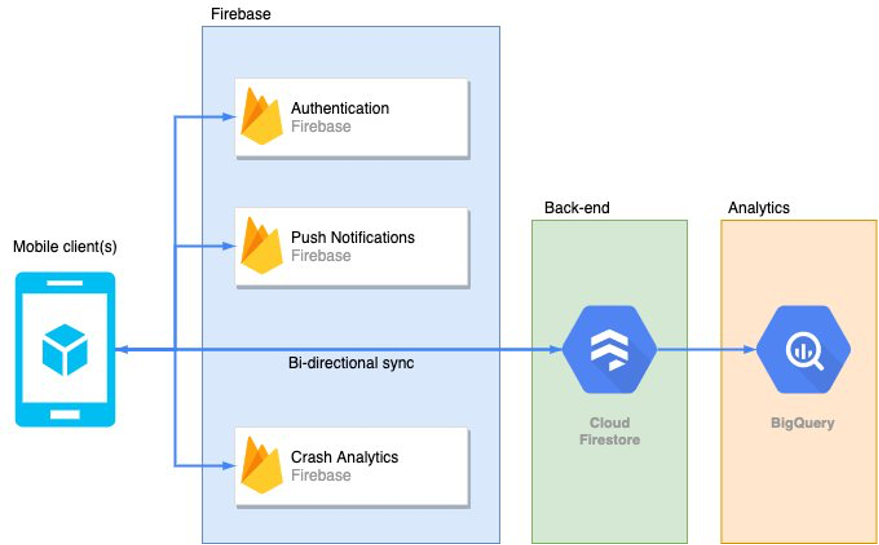
\includegraphics[width=0.7\textwidth]{img/figures/fig3-firebase-architecture.png}
  \caption{Diagrama de Arquitectura de Firebase. Fuente: Elaboración Propia.}
  \label{fig:firebase_architecture}
\end{figure}

En contraste, como se muestra en la \autoref{fig:amplify_architecture}, AWS adopta una arquitectura de tres capas, donde se separan de forma clara la capa de presentación, la lógica de negocio y la capa de datos. Esta organización modular permite un mayor control, escalabilidad y mantenibilidad del sistema, además de reducir significativamente el riesgo de exponer lógica de negocio crítica en el cliente.

En este enfoque, el cliente utiliza el SDK de AWS Amplify para comunicarse con los servicios del \textit{backend}, los cuales están implementados mediante funciones Lambda, las cuales pueden ser accedidas mediante una API REST usando Amazon API Gateway. De esta forma, se evita el acceso directo desde el frontend a las bases de datos o a la lógica sensible del negocio, incrementando la seguridad y permitiendo una evolución más controlada de la arquitectura.

\begin{figure}[H]
  \centering
  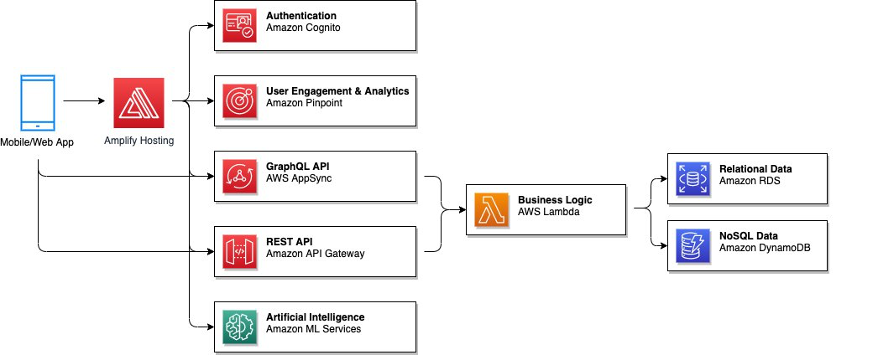
\includegraphics[width=1\textwidth]{img/figures/fig4-amplify-architecture.png}
  \caption{Diagrama de Arquitectura de AWS Amplify. Fuente: Elaboración Propia.}
  \label{fig:amplify_architecture}
\end{figure}

A diferencia de Firebase, donde todos los servicios están integrados dentro de una misma plataforma, AWS ofrece un enfoque más flexible y modular. Herramientas como AWS Amplify y el Amazon Cloud Development Kit (CDK) permiten definir, configurar e implementar servicios \textit{backend} de forma personalizada \cite{Michael2021}. Amplify proporciona un conjunto de herramientas para el desarrollo, incluyendo SDKs, generación automática de código y una pipeline DevOps que facilita la integración entre los servicios de AWS y las aplicaciones web o móviles \cite{Michael2021}.

Este enfoque permite construir arquitecturas completamente adaptadas a las necesidades del proyecto, seleccionando únicamente los servicios requeridos. Además, gracias al uso de Infraestructura como Código (IaC) mediante CDK o CloudFormation, es posible versionar, reutilizar y automatizar la configuración de los recursos, mejorando la mantenibilidad y escalabilidad del sistema.

Por otro lado, la migración de Firebase a AWS implica identificar servicios equivalentes que ofrezcan funcionalidades similares, pero con mayor flexibilidad y escalabilidad. La Tabla 1 presenta la correspondencia general entre servicios de Firebase y sus equivalentes en AWS.
